\section{Finite automata}
\lecture{3}{28/1}

\begin{definition}[]
    A \textbf{non-deterministic finite automaton} (NFA)
    is represented by a $5$-tuple
    $(Q, \Sigma, \Delta, q, F)$
    consisting of
    \begin{enumerate}
        \item a finite set of \emph{states} $Q$;
        \item a finite set of \emph{input symbols} $\Sigma$;
        \item a \emph{transition function}
            $\Delta: Q \times \Sigma \to \mathcal P(Q)$;
        \item an \emph{initial state} $q_0 \in Q$; and
        \item a set of \emph{accepting states} $F \subset Q$
    \end{enumerate}
\end{definition}

\begin{example}
    Consider the following NFA.
    \begin{center}
        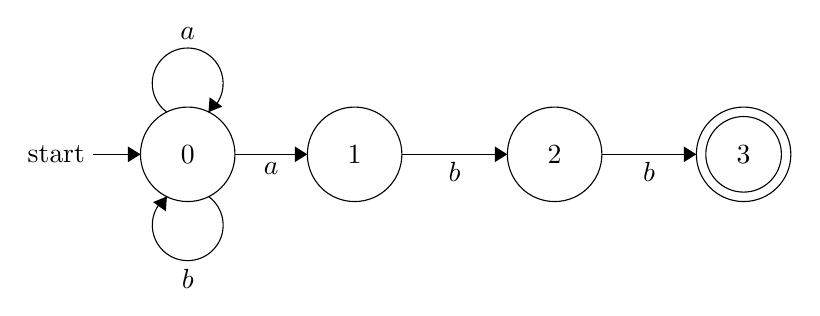
\begin{tikzpicture}[scale=0.2]
            \tikzstyle{every node}+=[inner sep=0pt]
            \draw [black] (11.9,-20.4) circle (3);
            \draw (11.9,-20.4) node {$0$};
            \draw [black] (22.5,-20.4) circle (3);
            \draw (22.5,-20.4) node {$1$};
            \draw [black] (35.2,-20.4) circle (3);
            \draw (35.2,-20.4) node {$2$};
            \draw [black] (47.2,-20.4) circle (3);
            \draw (47.2,-20.4) node {$3$};
            \draw [black] (47.2,-20.4) circle (2.4);
            \draw [black] (10.577,-17.72) arc (234:-54:2.25);
            \draw (11.9,-13.15) node [above] {$a$};
            \fill [black] (13.22,-17.72) -- (14.1,-17.37) -- (13.29,-16.78);
            \draw [black] (13.223,-23.08) arc (54:-234:2.25);
            \draw (11.9,-27.65) node [below] {$b$};
            \fill [black] (10.58,-23.08) -- (9.7,-23.43) -- (10.51,-24.02);
            \draw [black] (14.9,-20.4) -- (19.5,-20.4);
            \fill [black] (19.5,-20.4) -- (18.7,-19.9) -- (18.7,-20.9);
            \draw (17.2,-20.9) node [below] {$a$};
            \draw [black] (25.5,-20.4) -- (32.2,-20.4);
            \fill [black] (32.2,-20.4) -- (31.4,-19.9) -- (31.4,-20.9);
            \draw (28.85,-20.9) node [below] {$b$};
            \draw [black] (38.2,-20.4) -- (44.2,-20.4);
            \fill [black] (44.2,-20.4) -- (43.4,-19.9) -- (43.4,-20.9);
            \draw (41.2,-20.9) node [below] {$b$};
            \draw [black] (5.9,-20.4) -- (8.9,-20.4);
            \draw (5.4,-20.4) node [left] {start};
            \fill [black] (8.9,-20.4) -- (8.1,-19.9) -- (8.1,-20.9);
        \end{tikzpicture}
    \end{center}
    This automaton describes the language of strings containing $a$s and $b$s
    which have the suffix $abb$.
\end{example}

We say that a NFA \textbf{accepts} a string $x$ if there is a path from
the initial state to an accepting state, where $x$ is exactly the cocatenation
of edges along this path.
The \textbf{language} of an NFA is the set of strings that are accepted.

\begin{definition}[]
    A \textbf{deterministic finite automaton} (DFA)
    is represented as a $5$-tuple
    $(Q, \Sigma, \Delta, q_0, F)$
    consisting of
    \begin{enumerate}
        \item a finite set of states $Q$;
        \item a finite set of input symbols $\Sigma$;
        \item a transition function $\Delta: Q \times \Sigma \to Q$;
        \item an initial state $q_0 \in Q$; and
        \item a set of accepting states $F \subset Q$.
    \end{enumerate}
\end{definition}

Now the definition for a DFA and NFA are similar,
the difference is in the transition function.
At any given state, a DFA can only have \emph{one}
possible transition given a symbol.

\begin{example}
    Consider the following DFA.
    \begin{center}
        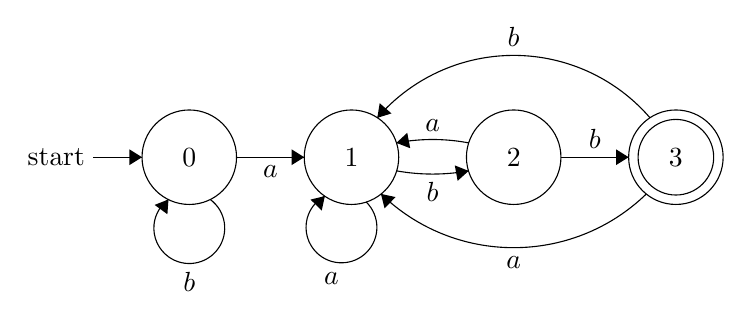
\begin{tikzpicture}[scale=0.2]
            \tikzstyle{every node}+=[inner sep=0pt]
            \draw [black] (13.1,-33.8) circle (3);
            \draw (13.1,-33.8) node {$0$};
            \draw [black] (23.4,-33.8) circle (3);
            \draw (23.4,-33.8) node {$1$};
            \draw [black] (33.7,-33.8) circle (3);
            \draw (33.7,-33.8) node {$2$};
            \draw [black] (44,-33.8) circle (3);
            \draw (44,-33.8) node {$3$};
            \draw [black] (44,-33.8) circle (2.4);
            \draw [black] (14.423,-36.48) arc (54:-234:2.25);
            \draw (13.1,-41.05) node [below] {$b$};
            \fill [black] (11.78,-36.48) -- (10.9,-36.83) -- (11.71,-37.42);
            \draw [black] (16.1,-33.8) -- (20.4,-33.8);
            \fill [black] (20.4,-33.8) -- (19.6,-33.3) -- (19.6,-34.3);
            \draw (18.25,-34.3) node [below] {$a$};
            \draw [black] (24.33,-36.64) arc (45.8699:-242.1301:2.25);
            \draw (22.12,-41.07) node [below] {$a$};
            \fill [black] (21.71,-36.27) -- (20.8,-36.49) -- (21.51,-37.19);
            \draw [black] (30.835,-34.667) arc (-79.81351:-100.18649:12.921);
            \fill [black] (30.84,-34.67) -- (29.96,-34.32) -- (30.14,-35.3);
            \draw (28.55,-35.37) node [below] {$b$};
            \draw [black] (36.7,-33.8) -- (41,-33.8);
            \fill [black] (41,-33.8) -- (40.2,-33.3) -- (40.2,-34.3);
            \draw (38.85,-33.3) node [above] {$b$};
            \draw [black] (26.251,-32.891) arc (100.72301:79.27699:12.355);
            \fill [black] (26.25,-32.89) -- (27.13,-33.23) -- (26.94,-32.25);
            \draw (28.55,-32.18) node [above] {$a$};
            \draw [black] (25.041,-31.299) arc (139.20811:40.79189:11.437);
            \fill [black] (25.04,-31.3) -- (25.94,-31.02) -- (25.19,-30.37);
            \draw (33.7,-26.83) node [above] {$b$};
            \draw [black] (42.125,-36.132) arc (-45.89294:-134.10706:12.105);
            \fill [black] (25.27,-36.13) -- (25.5,-37.05) -- (26.2,-36.33);
            \draw (33.7,-40.05) node [below] {$a$};
            \draw [black] (7,-33.8) -- (10.1,-33.8);
            \draw (6.5,-33.8) node [left] {start};
            \fill [black] (10.1,-33.8) -- (9.3,-33.3) -- (9.3,-34.3);
        \end{tikzpicture}
    \end{center}
    This DFA describes the same language as the NFA in the previous example.
\end{example}

\begin{theorem}[]
    Let $L$ be a formal language.
    Then there exists a NFA $M$
    such that $M$ recognises $L$.
\end{theorem}

\begin{theorem}[]
    Let $L$ be a formal language.
    If there exists a NFA $M$ such that $M$ recognises $L$,
    then there exists a DFA $M'$ such that $M'$ recognises $L$.
\end{theorem}

We will now see how to convert a regular expression to a NFA (and then to a DFA).
We do this process recursively.
Let $r,s,t$ be regular expressions and $N(s), N(t)$ represent
the NFA that accepts $s$ and $t$ respectively.
Then
\begin{enumerate}
    \item if $r = s \mid t$ we construct:
        \begin{center}
            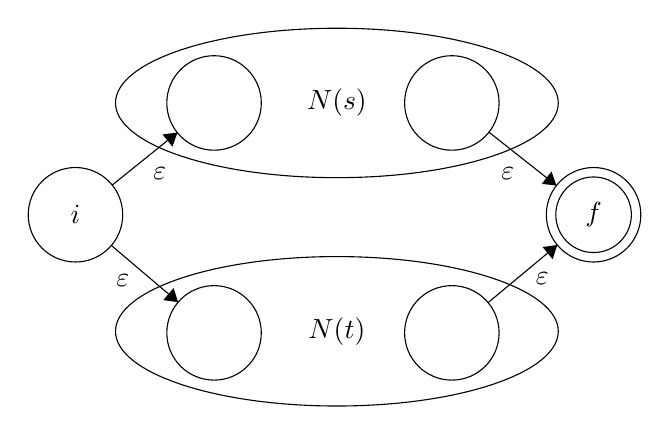
\begin{tikzpicture}[scale=0.2]
                \tikzstyle{every node}+=[inner sep=0pt]
                \draw [black] (12.4,-27.1) circle (3);
                \draw (12.4,-27.1) node {$i$};
                \draw [black] (21.2,-20) circle (3);
                \draw [black] (21.2,-34.6) circle (3);
                \draw [black] (36.3,-20) circle (3);
                \draw [black] (36.3,-34.6) circle (3);
                \draw [black] (45.3,-27.1) circle (3);
                \draw (45.3,-27.1) node {$f$};
                \draw [black] (45.3,-27.1) circle (2.4);
                \draw [black] (14.73,-25.22) -- (18.87,-21.88);
                \fill [black] (18.87,-21.88) -- (17.93,-22) -- (18.56,-22.78);
                \draw (17.75,-24.04) node [below] {$\varepsilon$};
                \draw [black] (14.68,-29.05) -- (18.92,-32.65);
                \fill [black] (18.92,-32.65) -- (18.63,-31.75) -- (17.98,-32.52);
                \draw (15.4,-30.84) node [below] {$\varepsilon$};
                \draw [black] (38.66,-21.86) -- (42.94,-25.24);
                \fill [black] (42.94,-25.24) -- (42.63,-24.35) -- (42.01,-25.14);
                \draw (39.85,-24.05) node [below] {$\varepsilon$};
                \draw [black] (38.6,-32.68) -- (43,-29.02);
                \fill [black] (43,-29.02) -- (42.06,-29.15) -- (42.7,-29.92);
                \draw (42.05,-30.74) node [below] {$\varepsilon$};
                \draw (29, -20) ellipse (400pt and 135pt) node {$N(s)$};
                \draw (29, -34.5) ellipse (400pt and 135pt) node {$N(t)$};
            \end{tikzpicture}
        \end{center}

    \item if $r = st$ we construct:
        \begin{center}
            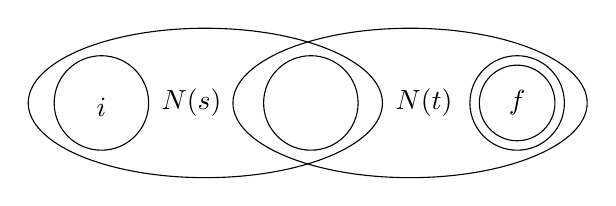
\begin{tikzpicture}[scale=0.2]
                \tikzstyle{every node}+=[inner sep=0pt]
                \draw [black] (12.4,-27.3) circle (3);
                \draw (12.4,-27.6) node {$i$};
                \draw [black] (25.7,-27.3) circle (3);
                \draw [black] (38.8,-27.3) circle (3);
                \draw (38.8,-27.3) node {$f$};
                \draw [black] (38.8,-27.3) circle (2.4);
                \draw (19, -27.3) ellipse (320pt and 135pt) node [xshift=-5pt] {$N(s)$};
                \draw (32, -27.3) ellipse (320pt and 135pt) node [xshift=5pt] {$N(t)$};
            \end{tikzpicture}
        \end{center}

    \item if $r = s^\star$ we construct:
        \begin{center}
            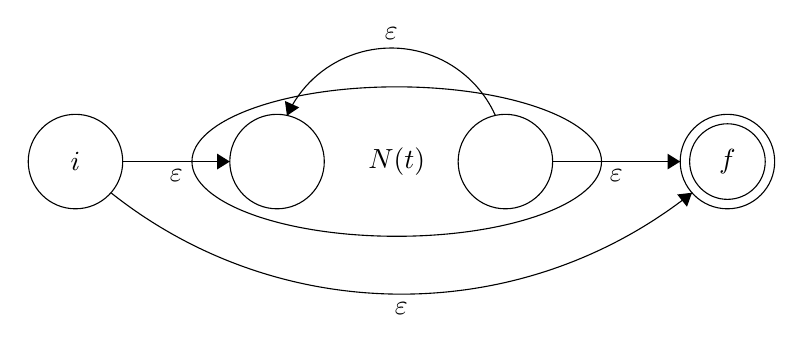
\begin{tikzpicture}[scale=0.2]
                \tikzstyle{every node}+=[inner sep=0pt]
                \draw [black] (16.6,-28.3) circle (3);
                \draw (16.6,-28.3) node {$i$};
                \draw [black] (29.4,-28.3) circle (3);
                \draw [black] (43.9,-28.3) circle (3);
                \draw [black] (58,-28.3) circle (3);
                \draw (58,-28.3) node {$f$};
                \draw [black] (58,-28.3) circle (2.4);
                \draw [black] (19.6,-28.3) -- (26.4,-28.3);
                \fill [black] (26.4,-28.3) -- (25.6,-27.8) -- (25.6,-28.8);
                \draw (23,-28.8) node [below] {$\varepsilon$};
                \draw [black] (30.029,-25.388) arc (155.96344:24.03656:7.25);
                \fill [black] (30.03,-25.39) -- (30.81,-24.86) -- (29.9,-24.45);
                \draw (36.65,-20.59) node [above] {$\varepsilon$};
                \draw [black] (55.75,-30.282) arc (-51.52983:-128.47017:29.657);
                \fill [black] (55.75,-30.28) -- (54.81,-30.39) -- (55.43,-31.17);
                \draw (37.3,-37.22) node [below] {$\varepsilon$};
                \draw [black] (46.9,-28.3) -- (55,-28.3);
                \fill [black] (55,-28.3) -- (54.2,-27.8) -- (54.2,-28.8);
                \draw (50.95,-28.8) node [below] {$\varepsilon$};
                \draw (37, -28.3) ellipse (370pt and 135pt) node {$N(t)$};
            \end{tikzpicture}
        \end{center}
\end{enumerate}

Now moving on to the transistion from a NFA to a DFA.
The idea here is to consider the states of our DFA
as a set of states possible from an input from the NFA.
This is best illustrates through an example.

\begin{example}
    Consider the following NFA.
    \begin{center}
        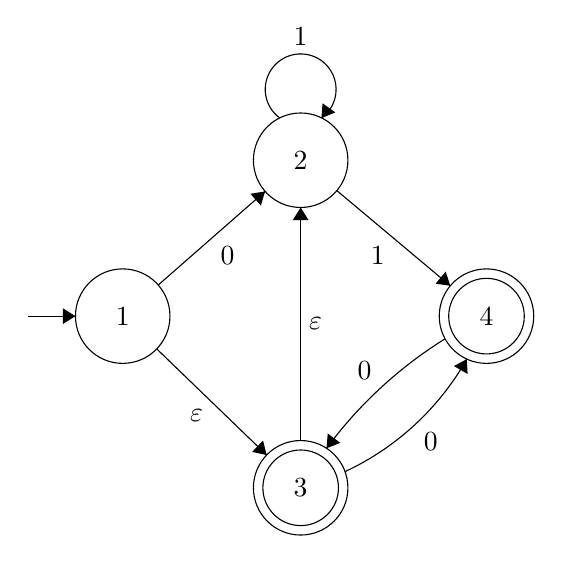
\begin{tikzpicture}[scale=0.2]
            \tikzstyle{every node}+=[inner sep=0pt]
            \draw [black] (9.9,-23.9) circle (3);
            \draw (9.9,-23.9) node {$1$};
            \draw [black] (21.2,-14) circle (3);
            \draw (21.2,-14) node {$2$};
            \draw [black] (33,-23.9) circle (3);
            \draw (33,-23.9) node {$4$};
            \draw [black] (33,-23.9) circle (2.4);
            \draw [black] (21.2,-34.8) circle (3);
            \draw (21.2,-34.8) node {$3$};
            \draw [black] (21.2,-34.8) circle (2.4);
            \draw [black] (3.9,-23.9) -- (6.9,-23.9);
            \fill [black] (6.9,-23.9) -- (6.1,-23.4) -- (6.1,-24.4);
            \draw [black] (12.16,-21.92) -- (18.94,-15.98);
            \fill [black] (18.94,-15.98) -- (18.01,-16.13) -- (18.67,-16.88);
            \draw (16.56,-19.44) node [below] {$0$};
            \draw [black] (12.06,-25.98) -- (19.04,-32.72);
            \fill [black] (19.04,-32.72) -- (18.81,-31.8) -- (18.12,-32.52);
            \draw (14.59,-29.83) node [below] {$\varepsilon$};
            \draw [black] (21.2,-31.8) -- (21.2,-17);
            \fill [black] (21.2,-17) -- (20.7,-17.8) -- (21.7,-17.8);
            \draw (21.7,-24.4) node [right] {$\varepsilon$};
            \draw [black] (31.755,-26.625) arc (-29.52938:-65.01152:17.288);
            \fill [black] (31.75,-26.63) -- (30.93,-27.07) -- (31.8,-27.57);
            \draw (29.46,-31.29) node [below] {$0$};
            \draw [black] (22.844,-32.292) arc (143.59225:121.86685:27.183);
            \fill [black] (22.84,-32.29) -- (23.72,-31.95) -- (22.92,-31.35);
            \draw (25.26,-27.97) node [above] {$0$};
            \draw [black] (23.5,-15.93) -- (30.7,-21.97);
            \fill [black] (30.7,-21.97) -- (30.41,-21.07) -- (29.77,-21.84);
            \draw (26.09,-19.44) node [below] {$1$};
            \draw [black] (19.877,-11.32) arc (234:-54:2.25);
            \draw (21.2,-6.75) node [above] {$1$};
            \fill [black] (22.52,-11.32) -- (23.4,-10.97) -- (22.59,-10.38);
        \end{tikzpicture}
    \end{center}
    The DFA equivalent to this is
    \begin{center}
        \footnotesize
        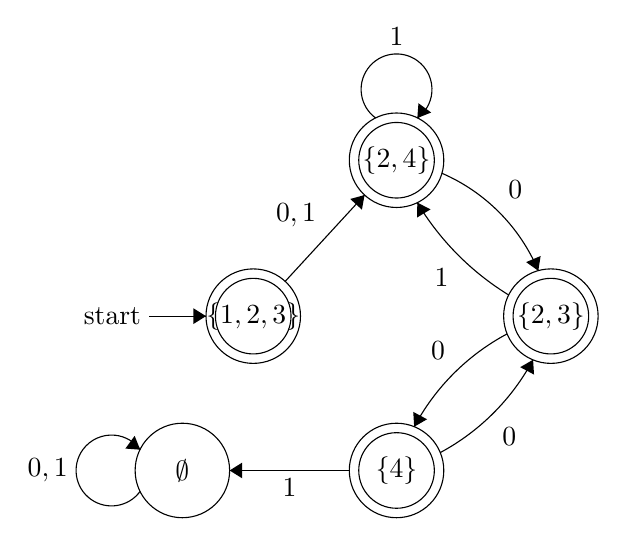
\begin{tikzpicture}[scale=0.2]
            \tikzstyle{every node}+=[inner sep=0pt]
            \draw [black] (23.1,-26.8) circle (3);
            \draw (23.1,-26.8) node {$\{1,2,3\}$};
            \draw [black] (23.1,-26.8) circle (2.4);
            \draw [black] (32.2,-16.9) circle (3);
            \draw (32.2,-16.9) node {$\{2,4\}$};
            \draw [black] (32.2,-16.9) circle (2.4);
            \draw [black] (42,-26.8) circle (3);
            \draw (42,-26.8) node {$\{2,3\}$};
            \draw [black] (42,-26.8) circle (2.4);
            \draw [black] (32.2,-36.6) circle (3);
            \draw (32.2,-36.6) node {$\{4\}$};
            \draw [black] (32.2,-36.6) circle (2.4);
            \draw [black] (18.6,-36.6) circle (3);
            \draw (18.6,-36.6) node {$\emptyset$};
            \draw [black] (16.5,-26.8) -- (20.1,-26.8);
            \draw (16,-26.8) node [left] {start};
            \fill [black] (20.1,-26.8) -- (19.3,-26.3) -- (19.3,-27.3);
            \draw [black] (29.2,-36.6) -- (21.6,-36.6);
            \fill [black] (21.6,-36.6) -- (22.4,-37.1) -- (22.4,-36.1);
            \draw (25.4,-37.1) node [below] {$1$};
            \draw [black] (15.92,-37.923) arc (-36:-324:2.25);
            \draw (11.35,-36.6) node [left] {$0,1$};
            \fill [black] (15.92,-35.28) -- (15.57,-34.4) -- (14.98,-35.21);
            \draw [black] (25.13,-24.59) -- (30.17,-19.11);
            \fill [black] (30.17,-19.11) -- (29.26,-19.36) -- (30,-20.04);
            \draw (27.12,-20.39) node [left] {$0,1$};
            \draw [black] (30.877,-14.22) arc (234:-54:2.25);
            \draw (32.2,-9.65) node [above] {$1$};
            \fill [black] (33.52,-14.22) -- (34.4,-13.87) -- (33.59,-13.28);
            \draw [black] (35.076,-17.725) arc (66.62105:22.79727:11.671);
            \fill [black] (41.2,-23.92) -- (41.35,-22.98) -- (40.43,-23.37);
            \draw (39.26,-18.75) node [right] {$0$};
            \draw [black] (39.321,-25.457) arc (-121.56483:-149.01685:17.391);
            \fill [black] (33.52,-19.59) -- (33.5,-20.54) -- (34.36,-20.02);
            \draw (35.54,-24.35) node [left] {$1$};
            \draw [black] (33.324,-33.825) arc (151.94351:118.05649:14.316);
            \fill [black] (33.32,-33.82) -- (34.14,-33.35) -- (33.26,-32.88);
            \draw (35.31,-28.96) node [left] {$0$};
            \draw [black] (40.866,-29.572) arc (-28.21171:-61.78829:14.43);
            \fill [black] (40.87,-29.57) -- (40.05,-30.04) -- (40.93,-30.51);
            \draw (38.88,-34.43) node [right] {$0$};
        \end{tikzpicture}
    \end{center}
\end{example}

\begin{definition}[Push-down automaton]
    A \textbf{push-down automaton} (PDA)
    is defined as a $7$-tuple
    $(Q, \Sigma, \Pi, \delta, q_0, Z, F)$
    consisting of
    \begin{enumerate}
        \item a finite set of \emph{states} Q;
        \item a finite set of \emph{input symbols} $\Sigma$;
        \item a finite set of \emph{stack symbols} $\Pi$;
        \item a \emph{transition relation} $\delta$;
        \item a \emph{start state} $q_0 \in Q$;
        \item an \emph{initial stack symbol} $Z \in \Pi$; and
        \item a set of \emph{accepting states} $F \subset Q$.
    \end{enumerate}
\end{definition}

\begin{remark}
    If, in every situation,
    at most one transition action is possible
    then the PDA is \emph{determinstic};
    otherwise, it is \emph{nondeterminstic}.
\end{remark}

\begin{example}
    Consider the following PDA.
    \begin{center}
        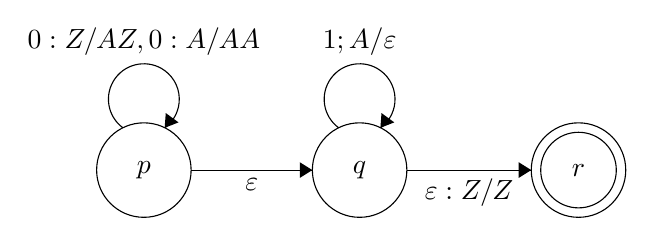
\begin{tikzpicture}[scale=0.2]
            \tikzstyle{every node}+=[inner sep=0pt]
            \draw [black] (11.7,-23.5) circle (3);
            \draw (11.7,-23.5) node {$p$};
            \draw [black] (25.4,-23.5) circle (3);
            \draw (25.4,-23.5) node {$q$};
            \draw [black] (39.3,-23.5) circle (3);
            \draw (39.3,-23.5) node {$r$};
            \draw [black] (39.3,-23.5) circle (2.4);
            \draw [black] (24.077,-20.82) arc (234:-54:2.25);
            \draw (25.4,-16.25) node [above] {$1;A/\varepsilon$};
            \fill [black] (26.72,-20.82) -- (27.6,-20.47) -- (26.79,-19.88);
            \draw [black] (10.377,-20.82) arc (234:-54:2.25);
            \draw (11.7,-16.25) node [above] {$0:Z/AZ,0:A/AA$};
            \fill [black] (13.02,-20.82) -- (13.9,-20.47) -- (13.09,-19.88);
            \draw [black] (14.7,-23.5) -- (22.4,-23.5);
            \fill [black] (22.4,-23.5) -- (21.6,-23) -- (21.6,-24);
            \draw (18.55,-24) node [below] {$\varepsilon$};
            \draw [black] (28.4,-23.5) -- (36.3,-23.5);
            \fill [black] (36.3,-23.5) -- (35.5,-23) -- (35.5,-24);
            \draw (32.35,-24) node [below] {$\varepsilon:Z/Z$};
        \end{tikzpicture}
    \end{center}
    In state $p$: for every $0$ we read we push $A$ on to the stack.
    In state $q$: for every $1$ we read we pop $A$ from the stack.
    Hence, this automaton accepts $L = \{0^n1^n: n \in \N\}$.
\end{example}

\begin{theorem}[]
    Let $L$ be a formal language.
    If there exists a PDA $P$ 
    such that $P$ recognises $L$,
    then $L$ is context-free.
\end{theorem}

\begin{theorem}[]
    There exists a formal language $L$
    such that there is exists a nondeterministic PDA $P$ 
    that recognises $L$
    but there does not exists a deterministic PDA $P'$
    that recognises $L$.
\end{theorem}
